\chapter{TESTING (Jakub Jędrzejczyk)}
\label{chap:Testing}

Testing of the application was performed in two stages: during development, and after the application was considered complete.
While testing during development was primarily focused on ensuring that individual features worked as intended, and the core of the application (the building process itself) could be carried out without issues, the post-development testing aimed to evaluate the application with the help of external testers.
They would be able to bring fresh perspectives to the experience, and point out any issues or inconveniences that may have been overlooked during development.

\section{Development Testing}

Testing during development consisted mostly of acceptance testing of individual features as they were implemented and regression testing to ensure that any new features did not break existing functionality \cite{anirbanSOFTWAREQUALITYASSURANCE2015}.

\subsection{Feature Testing}

Each component interaction was tested manually upon implementation to verify correct behavior.
This included:

\begin{itemize}
    \item \textbf{Grabbing and releasing:} Ensuring objects could be picked up and dropped reliably using the VR controllers;
    \item \textbf{Connection point detection:} Verifying that components would correctly identify valid mounting locations and snap into place when released within the acceptable tolerance;
    \item \textbf{Rotation mechanics:} Testing that both physical hand rotation and joystick-based fine adjustments worked as intended;
    \item \textbf{Audio and visual feedback:} Confirming that appropriate cues were triggered upon successful or failed placement attempts.
\end{itemize}

\subsection{Integration Testing}

After individual features were verified, integration testing was performed to ensure the complete PC building workflow could be executed from start to finish.
This involved building a complete PC configuration multiple times, verifying that:

\begin{itemize}
    \item Components could be installed in any order, but only valid connections could be made;
    \item The task list updated correctly as each step was completed;
    \item No component interactions interfered with previously placed parts.
\end{itemize}

\subsection{VR-Specific Considerations}

Given the nature of VR applications, additional testing focused on platform-specific concerns:

\begin{itemize}
    \item \textbf{Position translation:} Ensuring that real world hand movements accurately translated to in-app controller positions and to object manipulation;
    \item \textbf{Scale verification:} Ensuring component sizes matched real-world proportions to maintain immersion and educational accuracy during modelling.
\end{itemize}

\subsection{Limitations}

Due to time constraints and team size, formal unit testing and automated test suites were not implemented.
Testing was performed exclusively by the development team members, which may have introduced blind spots that were later identified during user testing (see Section \ref{sec:user-testing-results}).
Additionally, testing was mostly done on the team's PCs, with 

\section{User Testing}
\label{sec:user-testing}

\subsection{Methodology}

In order to more accurately evaluate user feedback, it was important to assess the user's prior knowledge of PC building.
To this end, a short survey was created, consisting of a few questions.
These questions were as follows:

\begin{itemize}
    \item Do you have a personal computer of the Desktop class?
    \begin{itemize}
        \item If yes, did you build it yourself?
        \begin{itemize}
            \item If yes, how many PCs (including that one) have you built?
            \item If yes, have you ever built a PC for someone else?
        \end{itemize}
        \item If no, what other computer-like devices (laptops, tablets, smartphones) do you own?
    \end{itemize}
    \item Have you ever helped someone else pick out components or fix an issue with their computer?
    \begin{itemize}
        \item If yes, how many times (more or less) did that happen?
    \end{itemize}
    \item Do you happen to interact with content regarding computer hardware (websites, YouTube channels, forums, etc.)?
    \begin{itemize}
        \item If yes, how often (a few times a week, once a week, once a month, less often than once a month) do you do that?
    \end{itemize}
    \item Other notes (optional, open-ended).
\end{itemize}

This would allow for categorizing users into one of three groups based on their prior knowledge of PC building:

\begin{itemize}
    \item No knowledge;
    \item Low knowledge;
    \item High knowledge.
\end{itemize}

Given these categories, having built three or more PCs for oneself or two (one for oneself and one for someone else) or regular interactions with computer hardware content (once a week or more often) would qualify as high knowledge.
Having built one or two PCs, helping someone else three or more times, or occasional interactions with computer hardware content (once a month or less often) would qualify as low knowledge.
Not meeting any of these criteria would qualify as no knowledge.

As the application is primarily targeted at users with little to no prior knowledge of PC building, so it's important to filter out feedback from more experienced users that may not accurately reflect the target audience's experience.
At the same time, their feedback, thanks to their experience, may provide valuable insights into potential improvements and missing features, so their feedback, categorized appropriately, is still valuable.

The testing itself consists of two parts: the user being presented with the developed application, tasked with building a PC using it, then being given a chance to complete the same task using a non-VR application (PC Building Simulator) for comparison.
The order of these parts was swapped for half of the testers in an attempt to reduce bias.

At the end of each of these parts, the user was given a questionnaire to fill out, consisting of Likert scale \cite{battertonLikertScaleWhat2017}
(strongly disagree, disagree, neutral, agree, strongly agree) and open-ended questions.
To avoid bias in answers which could be caused by all questions being positively phrased, some questions' phrasing was inverted.
After collecting the answers, the inverted questions' answers were flipped back for consistency.
These questions are as follows:

\begin{enumerate}
    \item After using the application, I:
    \begin{enumerate}
        \item feel more confident about building a desktop class PC;
        \item am more inclined to build my own PC in the future;
        \item don't feel like I've learned anything practical about PC building.
    \end{enumerate}
    \item Regarding the interface:
    \begin{enumerate}
        \item the simulator's interface was chaotic and not legible;
        \item it was easy to find the components I was looking for;
        \item instructions and hints were unclear or confusing;
        \item navigation in the simulator was intuitive;
        \item the virtual representation of components was unrealistic or misleading.
    \end{enumerate}
    \item Regarding the experience:
    \begin{enumerate}
        \item I knew what to do in the next step without looking for help;
        \item interactions with components were unnatural and frustrating;
        \item visual and audio feedback helped understand whether I was performing actions correctly;
        \item I often didn't know whether I was making progress or not.
    \end{enumerate}
\end{enumerate}

After completing both parts of the testing, the user was given a final questionnaire to fill out, comparing both experiences.
These questions are as follows:

\begin{enumerate}
    \setcounter{enumi}{3}
    \item Compared to PC Building Simulator:
    \begin{enumerate}
        \item I find PC Building Simulator to be more advanced than the VR simulator;
        \item I believe the VR simulator allows for a more immersive experience when it comes to building a PC;
        \item I prefer using the VR simulator over PC Building Simulator.
    \end{enumerate}
    \item Open-ended questions:
    \begin{enumerate}
        \item What was the hardest part of building a PC in the VR simulator?
        \item Which part of the interface was the least intuitive?
        \item What do you think is missing from the VR simulator?
        \item What helped you the most when building a PC in the VR simulator?
        \item Three things that you'd fix or change in the VR simulator?
    \end{enumerate}
\end{enumerate}

\subsection{Results}
\label{sec:user-testing-results}

The tests concluded with 7 participants, out of which 2 were categorized as having no prior knowledge of PC building, 2 as having low knowledge, and 3 as having high knowledge.
We recognize that this is too small of a sample size to be treated as statistically significant, moreover, most of the testers were at the very least acquaintances of the developers, with most being friends.
These facts limit the generalizability of the results, and we acknowledge the bias introduced by the aforementioned factors, however, in the limited timeframe available, it was not feasible to conduct a larger-scale study.
As such, the results should be treated as preliminary findings that may inform future, more comprehensive studies.

For the sake of legibility, each graph features the questions codes as per the list above, and the bar graphs feature Likert scale values represented numerically from 1 to 5, with 1 being "strongly disagree" and 5 being "strongly agree".

\begin{figure}[H]
	\centering
		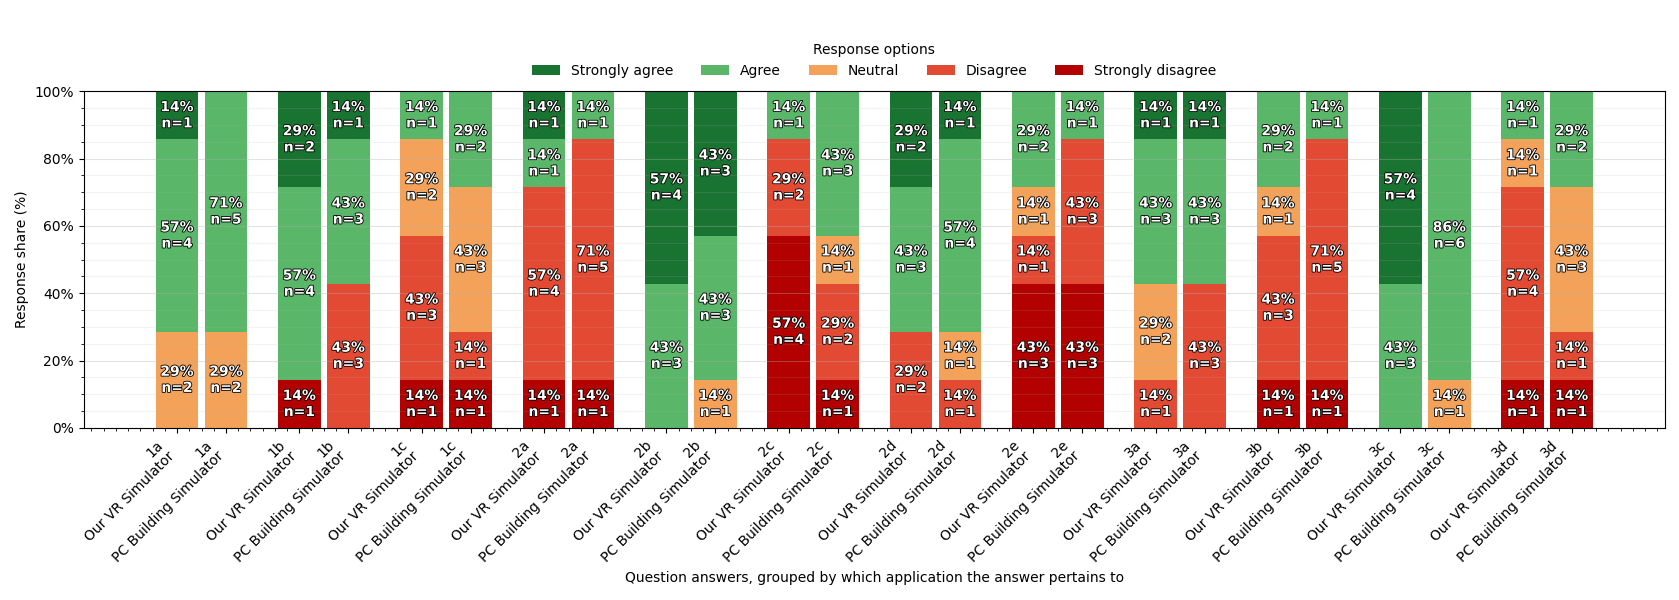
\includegraphics[width=1.0\textwidth]{testing/comparison_all_pairs_likert_grouped.png}
	\caption{Comparison of answers to application questionnaire, grouped by application.}
	\label{fig:ComparisonLikertGrouped}
\end{figure}

Figure \ref{fig:ComparisonLikertGrouped} shows the share of each of the options selected for each question, grouped by application used (VR simulator vs PC Building Simulator).

The answers to question 1a show that users felt slightly more confident and inclined to build their own PC after using the VR simulator, and 1b shows that they are more likely to build their own PC in the future after using the VR simulator as well.
Question 1c shows that users generally felt that they've learned more from the PC Building Simulator than the VR simulator, which is understandable given the much more true-to-life nature of the former.

Per question 2a, neither of the applications' interfaces were perceived as chaotic or illegible, though the VR simulator scored slightly worse.
Question 2b shows that the VR simulator's component search was slightly more effective, while 2c indicates that instructions and hints were notably clearer in the VR simulator than in the application.
Throughout the testing using PC Building Simulator, a few steps (e.g. installing the cooler which showed a rotating icon, while the user was expected to simply press the mouse button) proved to cause confusion.
Questions 2d and 2e show that the navigation in both of the applications was generally intuitive, with the VR simulator scoring slightly worse, and that visual representation of components was generally satisfactory in both applications, though the models in the VR simulator were perceived as slightly less realistic.
This is not surprising, given how the models were slightly simplified in the modelling process.

Regarding question 3a, it was generally easy for users to tell what to do next, though the straightforward list included in the VR simulator seems to be more helpful in this regard.
Question 3b indicates that interactions with components seemed slightly more frustrating in the VR simulator, which may partially be caused by most testers' lack of prior VR experience.
The VR simulator seems to provide more clear feedback on whether actions were performed correctly, as per question 3c.
This may be due to the fact that some of the more complex interactions that exist within PC Building Simulator (e.g. screwing in screws using a screwdriver) were skipped in the VR simulator for the sake of simplicity.
The testers were also less likely to tell whether they were making progress in the PC Building Simulator, as per question 3d, which may be due to the more complex nature of the application, and the much larger number of steps required to reach a functioning PC build.

\begin{figure}[H]
	\centering
		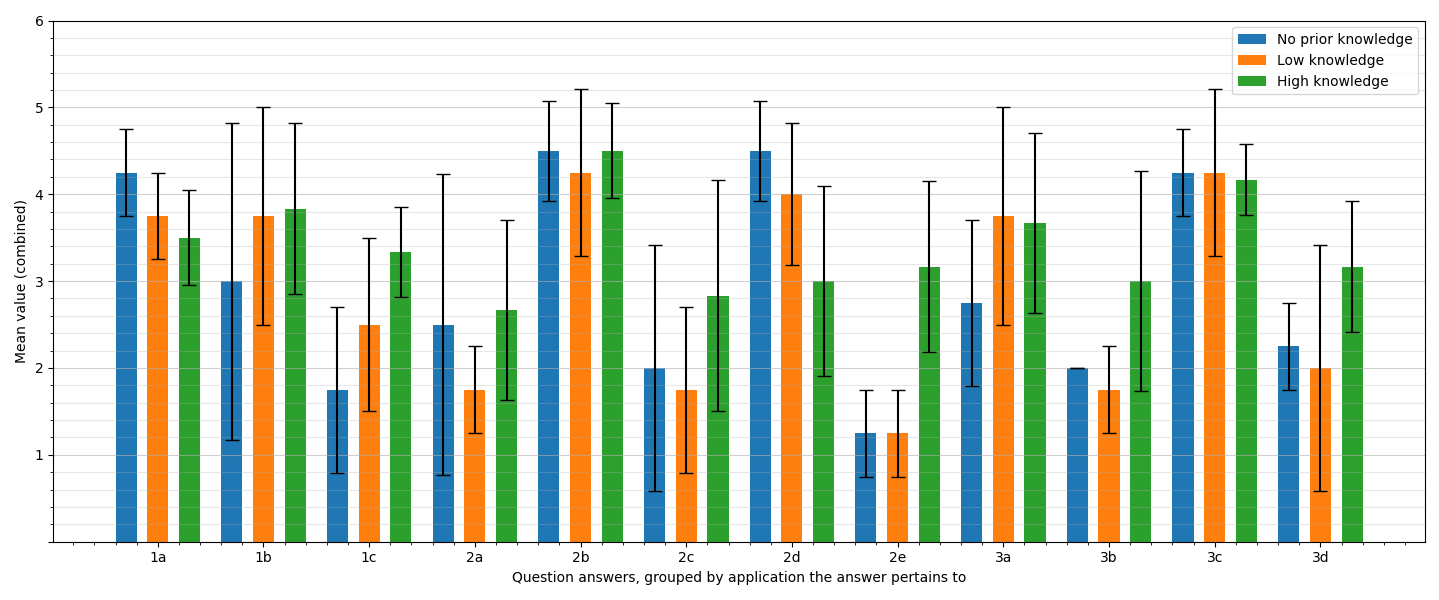
\includegraphics[width=1.0\textwidth]{testing/comparison_all_pairs_mean_grouped_by_class_combined.png}
	\caption{Comparison of mean values grouped by the classification of the user.}
	\label{fig:ComparisonMeanGroupedByClassCombined}
\end{figure}

Figure \ref{fig:ComparisonMeanGroupedByClassCombined} shows the mean answers to each question (with the standard deviation of the mean marked as well), grouped by the classification of the user (no knowledge, low knowledge, high knowledge), combining answers from both applications.
This allows for checking certain expectations regarding the users' prior knowledge.

For example, question 1a, checking whether the users felt more confident about building a PC, shows that the biggest growth in confidence was felt by users with no prior knowledge, while users with high knowledge felt only a slight increase in confidence.
Given the assumed inherent confidence in such users, this is an expected result.
While users with no prior knowledge felt largely neutral about building a PC in the future (1b), users with low and high knowledge (most likely already interested in PC building) felt more inclined to do so.
Similarly, users with no prior knowledge felt that they learned the most from the applications (1c), whereas users with high knowledge felt neutrally about any possible knowledge gain.

Questions 2a through 2c were expected to have similar results across all user groups, and this is indeed the case, though it's important to remark that the large deviations in no prior knowledge users' in 2a indicate that the two users in this group seemed to disagree on whether the interfaces were chaotic or not.
Also notable are the deviations in all groups in 2c, indicating that instructions and hints were perceived differently by different users.
Navigation intuitiveness (2d) was perceived worse with more experienced users, possibly caused by their preconceived notions of how such an application should work, but also possibly because their dislike of the controlling scheme, which will make itself obvious in the open-ended questions.
Visual representation of components (2e) was satisfactory for no prior knowledge and low knowledge users, while high knowledge users were slightly more critical of it.
This is not unexpected, given their experience with real-life components, and ability to critique details in the simplified models the VR simulator features.

Users with prior knowledge (low or high) generally knew what to do next without looking for help (3a), while users with no prior knowledge were more neutral on this matter.
This may indicate the need for more guidance for such users.
Interactions with components (3b) were perceived as more frustrating with highly knowledgeable users, possibly due to their prior experience with real components, and expectations of how such interactions should feel.
Visual and audio feedback (3c) was generally perceived as helpful across all user groups, while users with no prior knowledge were more likely to feel unsure about whether they were making progress (3d), indicating the need for more clear progress indicators for these users.

\begin{figure}[H]
	\centering
		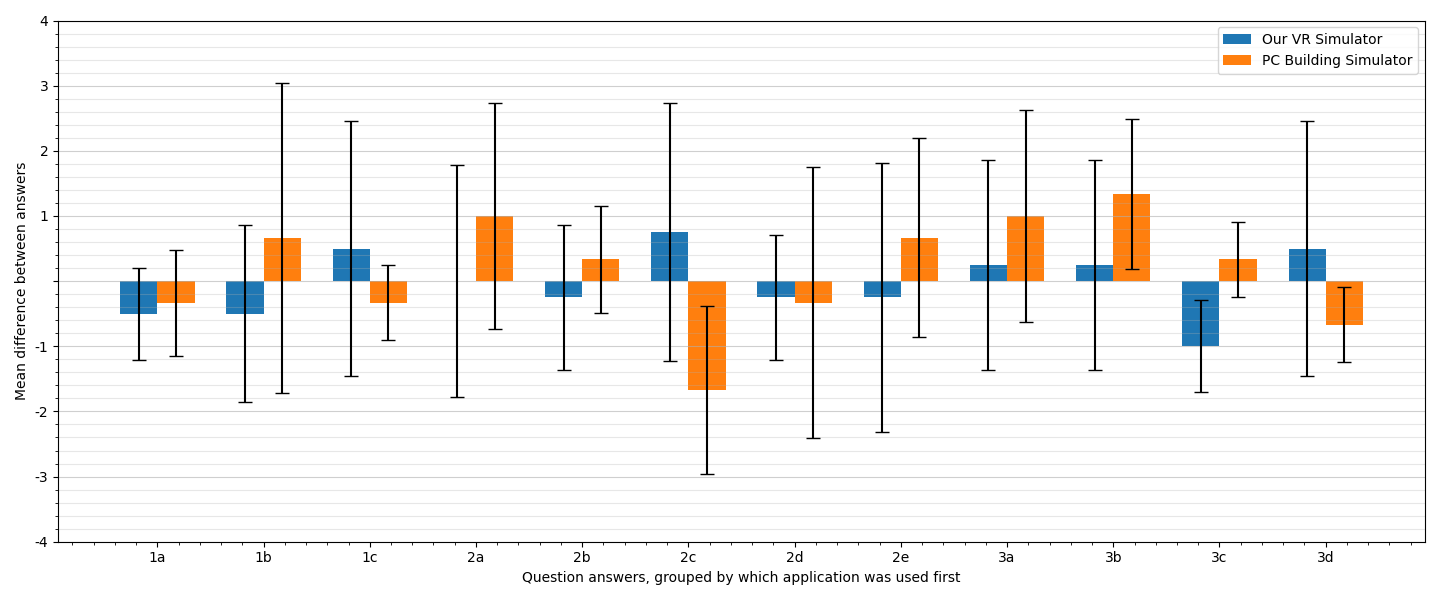
\includegraphics[width=1.0\textwidth]{testing/comparison_all_pairs_mean_grouped_delta.png}
	\caption{Comparison of differences between mean values grouped by the application used first.}
	\label{fig:ComparisonMeanGroupedDelta}
\end{figure}

As discussed previously, an important aspect of the testing methodology was the fact that the order of experiencing the two applications itself could influence the users' answers.
To analyze this effect, we compared the mean difference in answers between the second and the first application used, grouped by which application was used first (Figure \ref{fig:ComparisonMeanGroupedDelta}).
This graph can be interpreted as "adding" the value for each question 

Somewhat strangely, the confidence of building a PC (1a) seemed to decrease after using the second application, regardless of which application was used first.
This may be due to users realizing the complexity of PC building after experiencing both applications, though with such a small sample size, it's hard to draw definitive conclusions.
Using the VR simulator second seemed to build more inclination to build a PC in the future (1b), while using PC Building Simulator second seemed to decrease this inclination, though given the deviation in both groups, this result is not very reliable.
The knowledge gain (1c) seemed to generally be greater after using PC Building Simulator (as per the gain when using the VR simulator first, and loss when using PC Building Simulator first), which is expected given the more true-to-life nature of the application.

Users who used PC Building Simulator first seemed to find the VR simulator's interface less legible (2a), while experiencing PC Building Simulator second seemed to, on average, not affect this perception.
Finding components (2b) seemed to be easier after using the VR simulator, regardless of the order, though this difference is small.
Instructions and hints (2c) seemed to introduce more confusion in PC Building Simulator, regardless of the order, which may be caused by the previously discussed wider scope of that application.
Navigation intuitiveness (2d) seemed to be perceived as slightly worse after using either application second, though the effect is small.
Visual representation of components (2e) seemed to be perceived as slightly worse for the VR simulator, regardless of the order of applications used, which falls in line with the simplifications made in the modelling process.

Based on question 3a, it appears that using the VR simulator introduces more clarity about what action to take next, though given the nature of this question, and as knowledge can be gained from either application, seeing negative growth in either group would be unexpected.
Using the VR simulator seemed to introduce more frustrations "more reliably" (3b) when it was used second, which may be due to users being more critical after experiencing PC Building Simulator first.
Consistently with the previous questions, visual and audio feedback (3c) seemed to be perceived as more helpful after using the VR simulator, regardless of the order.
Finally, users seemed to feel more unsure about their progress (3d) in PC Building Simulator, regardless of the order of applications used.

The most consistent conclusion across these answers is that most likely due to the small sample size, the differing answers (as shown by large deviations) are much more prominent, making it hard to draw definitive conclusions about the effect of application order on users' answers.
Drawing conclusions about this bias is unreliable at best, and more extensive testing would be required to properly analyze this effect.

\begin{figure}[H]
	\centering
	\subfigure[]{
		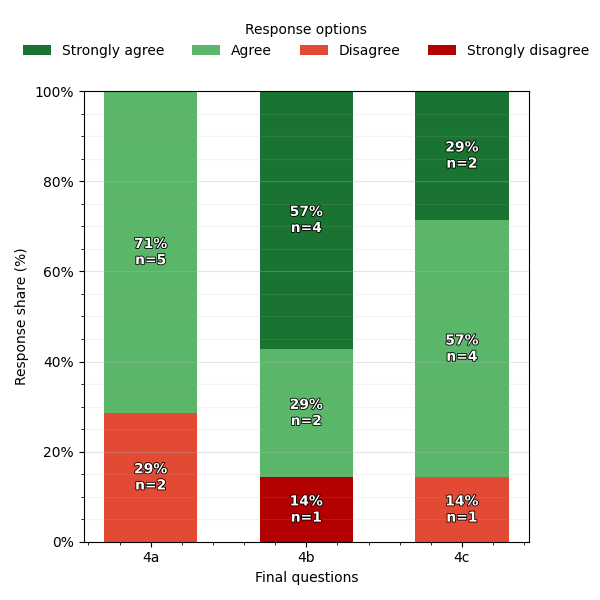
\includegraphics[width=0.45\textwidth]{testing/final_questions_likert.png}
		\label{fig:FinalQuestionsLikert}
	}%
	\hfil
	\subfigure[]{
		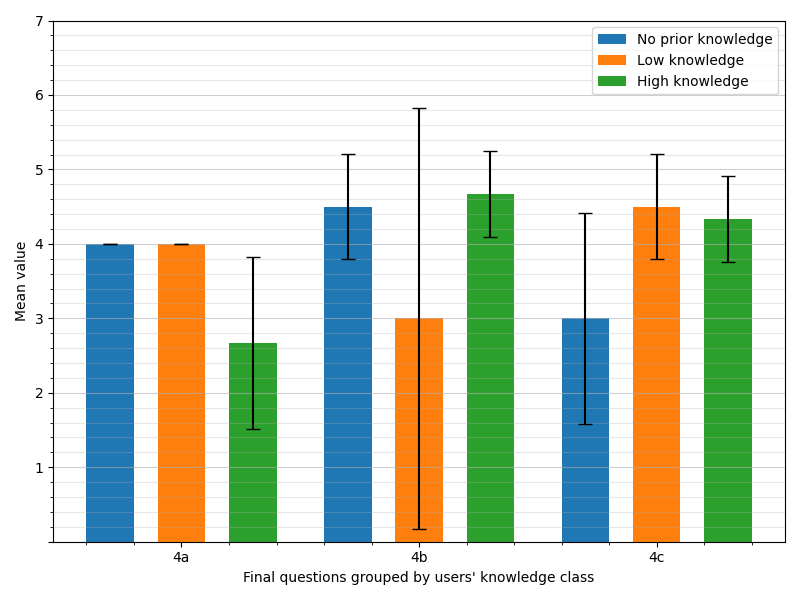
\includegraphics[width=0.45\textwidth]{testing/final_questions_mean_grouped_by_class.png}
		\label{fig:FinalQuestionsMeanGroupedClass}
	}
    \caption{Final questions analysis: (a) Likert scale answers share; (b) Mean answers grouped by user class.}%
\end{figure}

For the final questionnaire, the answers to the Likert scale questions are shown in Figure \ref{fig:FinalQuestionsLikert}, while the mean answers grouped by user class are shown in Figure \ref{fig:FinalQuestionsMeanGroupedClass}.

Answers to question 4a indicate that users generally found PC Building Simulator to be more advanced than the VR simulator, which is in line with expectations and is consistent with previous answers.
Question 4b shows that users found the VR simulator to be more immersive, which is to be expected given the nature of VR.
Notable however is the single outlier, which we believe to be a misunderstood answer (the user asked about the meaning of the word "immersive" and even after an explanation, seemed to answer contrary to discussions held together afterward).
Finally, question 4c shows that only one user did not prefer the VR simulator over PC Building Simulator, which is a promising result.
Perhaps of note is the fact that this user with no prior knowledge seemed to be much more interested in the customization aspect of PC Building Simulator, which given the limited component selection in the VR simulator, puts this answer into context.

The hardest part of building a PC in the VR simulator, as per question 5a, seems to be the object manipulation and controlling scheme, with 6 out of 7 users mentioning it in this question.
The single person who did not mention it chose RAM insertion as the hardest task instead.
Similarly, 5 out of 7 users mentioned the controlling scheme as the least intuitive part of the interface (5b), while the two remaining users declared that everything was intuitive.
Three people brought the control issue up again in question 5c regarding missing features in various forms (such as a way of stabilizing the user's hand, and guides for controls), while three others mentioned the lack of a wider component selection.
One person said that nothing was missing.
The most helpful aspect of the VR simulator (5d) seems to be the list of steps to complete, mentioned by 4 users.
Mentioned by one user were the audio feedback, object highlighting, and graphics card rotation, as well as the friend introducing the application.
The second to last in this list might be a misunderstanding from the user.

Lastly, the most asked for change (5e) was improving the controls, mentioned by all the users in a number of forms ("controller", "object rotation using the controller", "more intuitive object rotation", "predictability of object rotation").
Other suggestions included adding more components, particularly cables (mentioned by 3 people), increasing the model realism (2 people), adding more lighting (1 person), and decreasing the allowed rotational margin of error (1 person).
Not all users decided to list three changes.

These results, particularly the open-ended questions, provide valuable insights into potential improvements for the VR simulator.

The chosen controlling scheme seems to be a major pain point for users, indicating the need to rework it into something more intuitive and easier to use.
While this is something we recognize, it's also important to note that most of the users chose to conduct the majority of their object rotation using the controller joystick, while its intended use was for smaller adjustments or easy rotation of an object being inserted upside-down (e.g. the RAM stick not matching the slot orientation).
This indicates a need for better educating users on how to properly use the controls, as well as possibly reworking the controls themselves to better suit users' expectations.

The realism of the application models was another point of critique, particularly from more experienced users.
Because of the limited modelling capabilities and time constraints, the models were simplified to a degree, which may have affected the immersion for some users.
Certain details (such as the appropriately placed DDR groove in the RAM connectors on the motherboard's and RAM sticks' connectors) would be easy to add, while others (e.g. more detailed textures and better matching models) would require more time and effort.
Given the expectation of also increasing the component selection in the future, this might prove to be a challenge, though potentially presenting the current application to hardware manufacturers for collaboration might help alleviate this issue.

In spite of these critiques, the overall reception of the VR simulator proves that the immersive nature of VR is highly valued by users, and that the application has potential as an educational tool for PC building.
Currently, the educational value seems to be lacking due to simplifications and limited scope, but this could be improved in future iterations of the application.

\subsection{Summary and Recommendations}
\label{sec:user-testing-summary}

To summarize the key findings from user testing:

\begin{itemize}
    \item \textbf{User preference:} 6 out of 7 users (86\%) preferred the VR simulator over PC Building Simulator, validating the core concept of using VR for PC building education.
    \item \textbf{Immersion advantage:} The VR simulator was consistently rated as more immersive, confirming the hypothesis that VR provides a more engaging learning experience.
    \item \textbf{Target audience fit:} Users with no prior knowledge showed the greatest confidence gains, suggesting the application successfully serves its intended audience, though additional guidance mechanisms would be beneficial.
    \item \textbf{Guidance effectiveness:} The step-by-step task list was cited by 4 out of 7 users as the most helpful feature, validating this design decision.
\end{itemize}

Based on the feedback, we propose the following prioritized improvements:

\begin{enumerate}
    \item \textbf{High priority (short-term):}
    \begin{itemize}
        \item Rework the object rotation controls to be more intuitive, or provide a comprehensive tutorial on their use;
        \item Add clearer progress indicators for users with no prior knowledge.
    \end{itemize}
    \item \textbf{Medium priority (medium-term):}
    \begin{itemize}
        \item Improve model realism, particularly for connectors and textures;
        \item Add wider cable selection.
    \end{itemize}
    \item \textbf{Lower priority (long-term):}
    \begin{itemize}
        \item Expand component selection;
        \item Explore partnerships with hardware manufacturers for authentic models.
    \end{itemize}
\end{enumerate}

It should be noted that the limited sample size (n=7) and the testers' general lack of prior VR experience likely influenced some results, particularly regarding control frustrations.
Future studies should include a larger, more diverse sample with varying levels of VR familiarity to better isolate application-specific issues from general VR adaptation challenges.